\documentclass[11pt,a4paper]{article}
\usepackage[margin=2.4cm]{geometry}
\usepackage{amsmath,amssymb,mathtools,amsthm}
\usepackage[T1]{fontenc}
\usepackage{parskip}
\usepackage{tikz}
\usepackage[hidelinks]{hyperref}
\newcommand{\R}{\mathbb R}
\newcommand{\one}{\mathbf 1}
\newcommand{\dd}{\mathrm d}
\newcommand{\dlv}{\Sigma}
\newcommand{\ip}[2]{\langle #1,#2\rangle}
\newtheorem{lemma}{Lemma}
\renewcommand{\theequation}{R\arabic{equation}}
\begin{document}
\begin{center}
{\large\bfseries The code-book across two grids}\\[0.2em]
{\small The construction is due to Hans Buehler; written up by Magnus Wiese in the paper's notation, 3 October 2026.}
\end{center}

\section*{Summary}
If consecutive expiries live on different strike grids, the code-book becomes
\begin{equation}\label{eq:cb}
  A_j(\dlv^j)\,q^j=R_j\,q^{j-1},
\end{equation}
where $R_j$ splits each node of grid $j-1$ barycentrically onto the two grid-$j$ nodes that
bracket it. $R_j$ is constant while both grids are fixed, keeps mass and mean, and leaves
every price at a grid-$j$ strike unchanged. The paper's fixed common grid is $R_j=I$. The drift restriction is
unchanged, and the volatility recursion carries over with $\psi^{j-1}$ replaced by
$R_j\psi^{j-1}$.

\section{The operator}
Grid $j-1$ has nodes $y^m:=K^{j-1,m}$, grid $j$ has nodes $K^{j,i}$. Assume every $y^m$ lies in
$[K^{j,0},K^{j,N_j+1}]$ (automatic if both grids share the outer nodes, e.g.\ $0$ and a cap
$U$). If $K^{j,i}\le y^m\le K^{j,i+1}$, set
\begin{equation}\label{eq:R}
  (R_j)_{i,m}=\frac{K^{j,i+1}-y^m}{K^{j,i+1}-K^{j,i}},\qquad
  (R_j)_{i+1,m}=\frac{y^m-K^{j,i}}{K^{j,i+1}-K^{j,i}},
\end{equation}
and all other entries of column $m$ zero; if $y^m=K^{j,i}$, column $m$ is $e_i$. So
$R_j\in\R^{(N_j+2)\times(N_{j-1}+2)}$ has at most two non-zero entries per column.

\textbf{Example.} Both grids share the outer nodes $0$ and $U$. Old interior nodes
$80,90,100,110,120$, new $75,85,100,115,125$ (columns old, rows new):
\[
  R=\begin{pmatrix}
    1&0&0&0&0&0&0\\[1pt]
    0&\tfrac12&0&0&0&0&0\\[1pt]
    0&\tfrac12&\tfrac23&0&0&0&0\\[1pt]
    0&0&\tfrac13&1&\tfrac13&0&0\\[1pt]
    0&0&0&0&\tfrac23&\tfrac12&0\\[1pt]
    0&0&0&0&0&\tfrac12&0\\[1pt]
    0&0&0&0&0&0&1
  \end{pmatrix}
  \begin{matrix}\leftarrow0\\ \leftarrow75\\ \leftarrow85\\ \leftarrow100\\ \leftarrow115\\ \leftarrow125\\ \leftarrow U\end{matrix}
\]
with columns $0,80,90,100,110,120,U$.

\begin{figure}[H]\centering
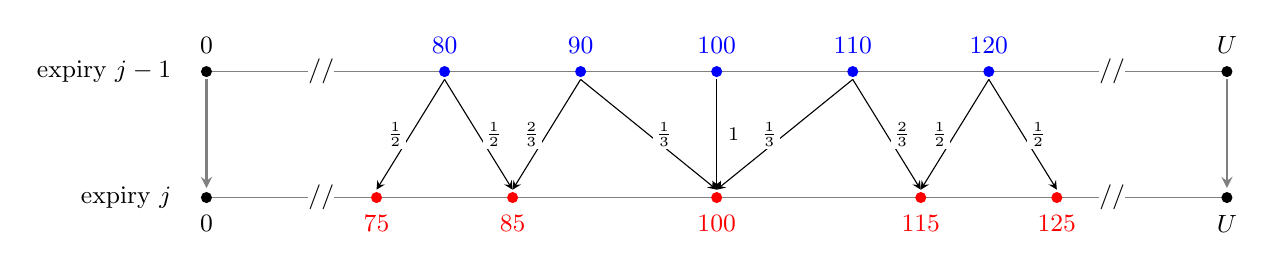
\begin{tikzpicture}[x=1.08cm,y=1cm,>=stealth]
\draw[gray] (0,1.6)--(1.2,1.6); \draw[gray] (1.5,1.6)--(10.5,1.6); \draw[gray] (10.8,1.6)--(12,1.6);
\node[anchor=east,font=\small] at (-0.3,1.6) {expiry $j-1$};
\node[font=\small] at (1.35,1.6) {//};
\node[font=\small] at (10.65,1.6) {//};
\draw[gray] (0,0)--(1.2,0); \draw[gray] (1.5,0)--(10.5,0); \draw[gray] (10.8,0)--(12,0);
\node[anchor=east,font=\small] at (-0.3,0) {expiry $j$};
\node[font=\small] at (1.35,0) {//};
\node[font=\small] at (10.65,0) {//};
\fill (0,1.6) circle (2pt); \fill (12,1.6) circle (2pt);
\fill (0,0) circle (2pt); \fill (12,0) circle (2pt);
\node[above,font=\small] at (0,1.7) {$0$}; \node[above,font=\small] at (12,1.7) {$U$};
\node[below,font=\small] at (0,-0.1) {$0$}; \node[below,font=\small] at (12,-0.1) {$U$};
\draw[->,thick,gray] (0,1.5)--(0,0.12); \draw[->,thick,gray] (12,1.5)--(12,0.12);
\fill[blue] (2.800,1.6) circle (2pt); \node[above,font=\small,blue] at (2.800,1.7) {80};
\fill[blue] (4.400,1.6) circle (2pt); \node[above,font=\small,blue] at (4.400,1.7) {90};
\fill[blue] (6.000,1.6) circle (2pt); \node[above,font=\small,blue] at (6.000,1.7) {100};
\fill[blue] (7.600,1.6) circle (2pt); \node[above,font=\small,blue] at (7.600,1.7) {110};
\fill[blue] (9.200,1.6) circle (2pt); \node[above,font=\small,blue] at (9.200,1.7) {120};
\fill[red] (2.000,0) circle (2pt); \node[below,font=\small,red] at (2.000,-0.1) {75};
\fill[red] (3.600,0) circle (2pt); \node[below,font=\small,red] at (3.600,-0.1) {85};
\fill[red] (6.000,0) circle (2pt); \node[below,font=\small,red] at (6.000,-0.1) {100};
\fill[red] (8.400,0) circle (2pt); \node[below,font=\small,red] at (8.400,-0.1) {115};
\fill[red] (10.000,0) circle (2pt); \node[below,font=\small,red] at (10.000,-0.1) {125};
\draw[->] (2.800,1.5)--(2.000,0.1);
\node[font=\scriptsize,fill=white,inner sep=1pt] at (2.220,0.8) {$\tfrac12$};
\draw[->] (2.800,1.5)--(3.600,0.1);
\node[font=\scriptsize,fill=white,inner sep=1pt] at (3.380,0.8) {$\tfrac12$};
\draw[->] (4.400,1.5)--(3.600,0.1);
\node[font=\scriptsize,fill=white,inner sep=1pt] at (3.820,0.8) {$\tfrac23$};
\draw[->] (4.400,1.5)--(6.000,0.1);
\node[font=\scriptsize,fill=white,inner sep=1pt] at (5.380,0.8) {$\tfrac13$};
\draw[->] (6.000,1.5)--(6.000,0.1);
\node[font=\scriptsize,fill=white,inner sep=1pt] at (6.200,0.8) {$1$};
\draw[->] (7.600,1.5)--(6.000,0.1);
\node[font=\scriptsize,fill=white,inner sep=1pt] at (6.620,0.8) {$\tfrac13$};
\draw[->] (7.600,1.5)--(8.400,0.1);
\node[font=\scriptsize,fill=white,inner sep=1pt] at (8.180,0.8) {$\tfrac23$};
\draw[->] (9.200,1.5)--(8.400,0.1);
\node[font=\scriptsize,fill=white,inner sep=1pt] at (8.620,0.8) {$\tfrac12$};
\draw[->] (9.200,1.5)--(10.000,0.1);
\node[font=\scriptsize,fill=white,inner sep=1pt] at (9.780,0.8) {$\tfrac12$};
\end{tikzpicture}
\caption{$R_j$ for two expiries. Each old node (blue) sends its mass to the two new nodes (red) around it, with the barycentric weights; $100$ is on both grids, and the shared outer nodes $0$ and $U$ map to themselves. The new grid has the same number of nodes, with wider spacing.}
\end{figure}

\textbf{Numerically.} Old masses and their image:
\[
  q=(0,\,0.1,\,0.2,\,0.4,\,0.2,\,0.1,\,0),\qquad
  Rq=(0,\,0.05,\,0.18\overline3,\,0.5\overline3,\,0.18\overline3,\,0.05,\,0),
\]
with mass $1$ and mean $100$, as before.

\section{Properties}
\begin{lemma}\label{lem:R}
\begin{enumerate}
\item $R_j\ge0$, $\one^{\!\top}R_j=\one^{\!\top}$ and $(K^{j})^{\!\top}R_j=(K^{j-1})^{\!\top}$:
  mass and mean are kept.
\item Splitting does not change any price on the new grid. Write $C[q](K)$ for the call
  price of a density $q$ at strike $K$. Then
  \[
    C[R_jq](K)=C[q](K)\qquad\text{for every strike $K$ of grid $j$.}
  \]
\end{enumerate}
\end{lemma}

\section{The code-book \eqref{eq:cb} and what carries over}
\begin{itemize}
\item \textbf{Static.} Given $\dlv^j>0$, $q^j=P_jR_jq^{j-1}$ ($P_j=A_j(\dlv^j)^{-1}$) is a
  probability vector with mean $S$ (Lemma~\ref{lem:R}(1)).
\item \textbf{Why $R_j$ acts on $q^{j-1}$.} Projecting $q^j$ onto grid $j-1$ instead would merge
  nodes, so $q^j$ would not be determined by the code-book.
\item \textbf{Drift restriction: unchanged.} $R_j$ is constant and $q^{j-1}$ is a martingale, so
  $R_jq^{j-1}$ has no drift; the $\dd t$-part is as before and
  $\alpha^{j,i}=-\ip{\eta^{j,i}}{\beta^{j,i}}$. $R_j$ need not be invertible; injectivity is
  still only needed for $\widehat G_j$.
\item \textbf{Volatility recursion:}
  $A_j(\dlv^j)\,\psi^j=R_j\psi^{j-1}-G_j(q^j)\,\beta^j$.
\item \textbf{Handover at expiry:} if the front settles on its node $k$, the new front
  $P_2R_2e_k$ is strictly positive.
\end{itemize}

\end{document}
